\documentclass[12pt,a4paper]{article}

% Packages
\usepackage[utf8]{inputenc}
\usepackage[portuguese]{babel}
\usepackage{graphicx}
\usepackage{geometry}
\usepackage{hyperref}
\usepackage{fancyhdr}
\usepackage{titlesec}
\usepackage{enumitem}
\usepackage{float}

% Page geometry
\geometry{
    top=2.5cm,
    bottom=2.5cm,
    left=2.5cm,
    right=2.5cm
}

% Hyperref setup
\hypersetup{
    colorlinks=true,
    linkcolor=black,
    urlcolor=blue,
    citecolor=black
}

% Title formatting
\titleformat{\section}{\large\bfseries}{\thesection.}{1em}{}
\titleformat{\subsection}{\normalsize\bfseries}{\thesubsection.}{1em}{}

\begin{document}

% Title page
\begin{titlepage}
    \centering
    \vspace*{1cm}
    
    {\Large \textbf{Instituto Superior de Engenharia de Lisboa}}\\[0.5cm]
    
    {\large Departamento de Engenharia Eletrónica e Telecomunicações e de Computadores (DEETC)}\\[1cm]
    
    {\large Mestrado em Engenharia Informática e de Computadores}\\[2cm]
    
    {\LARGE \textbf{FINAL PROJECT - A1}}\\[1.5cm]
    
    {\Large Aprendizagem e Mineração de Dados (AMD)}\\[0.3cm]
    {\large 1º Semestre -- 2025/2026}\\[0.8cm]
    
    
\includegraphics[width=0.8\textwidth]{figures/01_ISEL-Logotipo-RGB_Horizontal-Compacto-900.png}\\[0.8cm]
    
    \vfill
    
    {\large \textbf{Autores:}}\\[0.2cm]
    {\large
        Florin Sofinet (A46608)\\
        Diogo Guerra (A49149)\\
        Nuno Silva (A53976)
    }
    
    \vfill
    
    {\large \today}
    
\end{titlepage}

% Table of contents
\tableofcontents
\newpage

% Main content
\section{Introdução}

Este laboratório tem como objetivo explorar métodos de avaliação de modelos de Machine Learning, combinando capacidades programáticas de Python com ferramentas de outras bibliotecas e do ambiente do Orange Data Mining.

Ao longo do trabalho, serão analisadas diversas técnicas de divisão de dados, métodos de amostragem, bootstrap, métricas de desempenho e construção de classificadores.

\section{Análise do dataset e da descrição}

O primeiro exercício consistiu na análise detalhada do ficheiro de dados original (\texttt{dataset\_long\_name\_ORIGINAL.csv}) e da respetiva descrição (\texttt{dataset\_description.txt}), identificando o significado de cada atributo, o objetivo da classificação, o número de instâncias, eventuais valores em falta e a distribuição das classes.

\subsection{Origem e contexto do dataset}

O dataset utilizado provém do \textit{UCI Machine Learning Repository} e contém descrições de amostras correspondentes a 23 espécies de cogumelos com lamelas das famílias Agaricus e Lepiota. Os dados foram extraídos do \textit{Audubon Society Field Guide to North American Mushrooms} (1981).

\subsection{Objetivo da classificação}

Cada amostra de cogumelo é classificada em uma das seguintes categorias:
\begin{itemize}
    \item \textbf{Edible} (comestível) -- cogumelos seguros para consumo
    \item \textbf{Poisonous} (venenoso) -- cogumelos tóxicos ou de comestibilidade desconhecida
\end{itemize}

\subsection{Características do dataset}

O dataset apresenta as seguintes características principais:

\begin{itemize}
    \item \textbf{Número de instâncias:} 8416 amostras
    \item \textbf{Número de atributos:} 22 atributos nominais (categóricos)
    \item \textbf{Atributo de classe:} \texttt{class} (EDIBLE ou POISONOUS)
    \item \textbf{Valores em falta:} 2480 valores ausentes (representados por ``?''), todos no atributo \#11 (\texttt{stalk-root})
\end{itemize}

\subsection{Distribuição das classes}

A distribuição das classes no dataset é relativamente equilibrada:

\begin{itemize}
    \item \textbf{Edible:} 4488 instâncias (53.33\%)
    \item \textbf{Poisonous:} 3928 instâncias (46.67\%)
\end{itemize}

Através de ferramentas de análise no Visual Studio Code, confirmou-se que o dataset contém exatamente 8416 instâncias (excluindo o cabeçalho), das quais 4488 são da classe \textit{edible} e 3928 da classe \textit{poisonous}.

\subsection{Atributos do dataset}

O dataset contém 22 atributos descritivos, todos nominais:

\begin{enumerate}
    \item \texttt{cap-shape} -- forma do chapéu (bell, conical, convex, flat, knobbed, sunken)
    \item \texttt{cap-surface} -- superfície do chapéu (fibrous, grooves, scaly, smooth)
    \item \texttt{cap-color} -- cor do chapéu (brown, buff, cinnamon, gray, green, pink, purple, red, white, yellow)
    \item \texttt{bruises} -- presença de hematomas (bruises, no)
    \item \texttt{odor} -- odor (almond, anise, creosote, fishy, foul, musty, none, pungent, spicy)
    \item \texttt{gill-attachment} -- tipo de fixação das lamelas (attached, free)
    \item \texttt{gill-spacing} -- espaçamento das lamelas (close, crowded)
    \item \texttt{gill-size} -- tamanho das lamelas (broad, narrow)
    \item \texttt{gill-color} -- cor das lamelas (10 valores possíveis)
    \item \texttt{stalk-shape} -- forma do caule (enlarging, tapering)
    \item \texttt{stalk-root} -- raiz do caule (bulbous, club, equal, rooted, missing)
    \item \texttt{stalk-surface-above-ring} -- superfície do caule acima do anel
    \item \texttt{stalk-surface-below-ring} -- superfície do caule abaixo do anel
    \item \texttt{stalk-color-above-ring} -- cor do caule acima do anel
    \item \texttt{stalk-color-below-ring} -- cor do caule abaixo do anel
    \item \texttt{veil-type} -- tipo de véu (partial)
    \item \texttt{veil-color} -- cor do véu (brown, orange, white, yellow)
    \item \texttt{ring-number} -- número de anéis (none, one, two)
    \item \texttt{ring-type} -- tipo de anel (8 valores possíveis)
    \item \texttt{spore-print-color} -- cor da impressão dos esporos (9 valores possíveis)
    \item \texttt{population} -- tipo de população (abundant, clustered, numerous, scattered, several, solitary)
    \item \texttt{habitat} -- habitat (grasses, leaves, meadows, paths, urban, waste, woods)
\end{enumerate}

\section{Transformação para formato .tab (Orange)}

O segundo exercício consistiu na transformação do dataset original (\texttt{dataset\_long\_name\_ORIGINAL.csv}) para o formato \texttt{.tab}, que é o formato nativo utilizado pelo Orange Data Mining. Este formato permite uma melhor integração com as ferramentas de análise e visualização do Orange.

\subsection{Método de transformação}

Para realizar a conversão, utilizou-se um script Python simples (\texttt{dataset\_converter.py}) que aproveita a biblioteca Orange para carregar o ficheiro CSV e convertê-lo automaticamente para o formato \texttt{.tab}:

\begin{verbatim}
import Orange

# Load CSV
data = Orange.data.Table("dataset_long_name_ORIGINAL.csv")

# Save as TAB
data.save("dataset_long_name_CONVERTED.tab")
\end{verbatim}

Este método é preferível à conversão manual porque:
\begin{itemize}
    \item Preserva corretamente os tipos de dados dos atributos
    \item Mantém a estrutura e metadados necessários para o Orange
    \item Garante compatibilidade total com o ambiente Orange Data Mining
    \item É reprodutível e automatizável
\end{itemize}

\subsection{Formato .tab do Orange}

O formato \texttt{.tab} do Orange é uma variante do formato TSV (Tab-Separated Values) que inclui três linhas de cabeçalho:
\begin{enumerate}
    \item \textbf{Linha 1:} Nomes dos atributos
    \item \textbf{Linha 2:} Tipos/flags dos atributos (ex: discrete, continuous, class, meta)
    \item \textbf{Linha 3:} Valores possíveis para atributos discretos
    \item \textbf{Linhas seguintes:} Dados das instâncias
\end{enumerate}

\subsection{Configuração da variável de classe}

Durante o processamento do dataset convertido, foi necessário ajustar a configuração para garantir que o atributo \texttt{class} fosse corretamente identificado como a variável de classe (target). Isto foi feito programaticamente no ficheiro \texttt{classifier\_handler.py}:

\begin{verbatim}
# If 'class' is not the class variable, set it manually
if self.data.domain.class_var is None:
    class_attr = None
    for attr in self.data.domain.attributes:
        if attr.name == 'class':
            class_attr = attr
            break
    
    if class_attr:
        new_attrs = [attr for attr in self.data.domain.attributes 
                     if attr.name != 'class']
        new_domain = Orange.data.Domain(new_attrs, class_attr)
        self.data = self.data.transform(new_domain)
\end{verbatim}

Esta configuração garante que o atributo \texttt{class} seja tratado como a variável dependente nas análises subsequentes, permitindo que os algoritmos de classificação funcionem corretamente.

\subsection{Ficheiro resultante}

O ficheiro resultante (\texttt{dataset\_long\_name\_CONVERTED.tab}) mantém todas as 8416 instâncias e os 22 atributos originais, com o atributo \texttt{class} corretamente configurado como variável de classe. Este ficheiro foi utilizado como base para os exercícios seguintes, nomeadamente para a aplicação do algoritmo 1R e para as análises no Orange Data Mining.

\section{Aplicação do classificador 1R}

O terceiro exercício consistiu na aplicação do algoritmo 1R (\textit{One Rule}) ao dataset de cogumelos. O algoritmo 1R é um classificador simples mas eficaz que seleciona o atributo único que melhor classifica os dados, criando regras baseadas nos valores desse atributo.

\subsection{Implementação do algoritmo 1R}

O algoritmo 1R foi implementado em Python utilizando a biblioteca Orange. A implementação encontra-se no ficheiro \texttt{one\_rule.py} e segue os seguintes passos:

\begin{enumerate}
    \item Para cada atributo discreto no dataset:
    \begin{itemize}
        \item Para cada valor possível do atributo, identifica a classe mais frequente
        \item Calcula o número de erros (instâncias que não pertencem à classe mais frequente)
    \end{itemize}
    \item Seleciona o atributo com o menor número total de erros
    \item Retorna o atributo selecionado, a regra correspondente e a taxa de erro
\end{enumerate}

\subsection{Execução e resultados}

A aplicação do algoritmo 1R foi realizada através do script \texttt{classifier\_handler.py}, que:
\begin{itemize}
    \item Carrega o dataset convertido (\texttt{dataset\_long\_name\_CONVERTED.tab})
    \item Divide os dados em conjunto de treino (80\%) e teste (20\%)
    \item Aplica o algoritmo 1R ao conjunto de treino
    \item Gera estatísticas detalhadas para cada combinação (atributo, valor, classe)
\end{itemize}

O algoritmo foi executado com sucesso, gerando o ficheiro \texttt{oneR\_OUTPUT.txt} com o formato especificado.

\subsection{Atributo selecionado: odor}

O algoritmo 1R selecionou o atributo \textbf{odor} (odor do cogumelo) como o melhor preditor único para a classificação. Este resultado é altamente significativo e intuitivo do ponto de vista biológico, uma vez que o odor é frequentemente um indicador importante da comestibilidade de cogumelos.

\subsection{Taxa de erro}

A taxa de erro obtida foi de apenas \textbf{0.0143} (1.43\%), o que demonstra que o atributo \texttt{odor} sozinho é capaz de classificar corretamente 98.57\% das instâncias do conjunto de treino. Este resultado excepcionalmente bom sugere que o odor é um preditor extremamente forte para este dataset.

\subsection{Regras geradas}

As regras geradas pelo algoritmo 1R para o atributo \texttt{odor} são apresentadas no ficheiro \texttt{oneR\_OUTPUT.txt} no formato especificado:

\texttt{(attr, valueAttr, valueTarget) : (error, total)}

\noindent onde:
\begin{itemize}
    \item \texttt{attr} -- nome do atributo selecionado (odor)
    \item \texttt{valueAttr} -- cada valor possível do atributo odor
    \item \texttt{valueTarget} -- cada classe (EDIBLE ou POISONOUS)
    \item \texttt{error} -- número de classificações incorretas para essa combinação
    \item \texttt{total} -- número total de instâncias para essa combinação
\end{itemize}

\subsection{Análise detalhada dos resultados}

Os resultados completos obtidos do ficheiro \texttt{oneR\_OUTPUT.txt} são:

\begin{verbatim}
Selected attribute: odor
Error rate: 0.0143

(odor, ALMOND, EDIBLE) : (0, 308)
(odor, ANISE, EDIBLE) : (0, 304)
(odor, CREOSOTE, POISONOUS) : (0, 153)
(odor, FISHY, POISONOUS) : (0, 472)
(odor, FOUL, POISONOUS) : (0, 1724)
(odor, MUSTY, POISONOUS) : (0, 35)
(odor, NONE, EDIBLE) : (0, 2957)
(odor, NONE, POISONOUS) : (96, 96)
(odor, PUNGENT, POISONOUS) : (0, 218)
(odor, SPICY, POISONOUS) : (0, 465)
\end{verbatim}

\subsection{Interpretação das regras}

A análise dos resultados revela padrões claros:

\begin{itemize}
    \item \textbf{Odores associados a cogumelos comestíveis:}
    \begin{itemize}
        \item ALMOND (amêndoa): 308 instâncias, todas EDIBLE (0 erros)
        \item ANISE (anis): 304 instâncias, todas EDIBLE (0 erros)
        \item NONE (sem odor): 2957 instâncias EDIBLE, classificadas corretamente
    \end{itemize}
    
    \item \textbf{Odores associados a cogumelos venenosos:}
    \begin{itemize}
        \item CREOSOTE: 153 instâncias, todas POISONOUS (0 erros)
        \item FISHY (peixe): 472 instâncias, todas POISONOUS (0 erros)
        \item FOUL (fétido): 1724 instâncias, todas POISONOUS (0 erros)
        \item MUSTY (mofo): 35 instâncias, todas POISONOUS (0 erros)
        \item PUNGENT (pungente): 218 instâncias, todas POISONOUS (0 erros)
        \item SPICY (picante): 465 instâncias, todas POISONOUS (0 erros)
    \end{itemize}
    
    \item \textbf{Única fonte de erros:}
    \begin{itemize}
        \item NONE (sem odor) + POISONOUS: 96 instâncias mal classificadas
        \item Estes cogumelos venenosos sem odor característico foram incorretamente classificados como EDIBLE pela regra, uma vez que a maioria dos cogumelos sem odor (2957) são comestíveis
    \end{itemize}
\end{itemize}

\subsection{Conclusões do exercício 1R}

O algoritmo 1R demonstrou que:
\begin{enumerate}
    \item O atributo \texttt{odor} é um preditor excepcionalmente forte para a classificação de cogumelos
    \item Cogumelos com odores como ALMOND ou ANISE são consistentemente comestíveis
    \item Cogumelos com odores desagradáveis (FOUL, FISHY, MUSTY, PUNGENT, SPICY) são consistentemente venenosos
    \item A única ambiguidade significativa ocorre com cogumelos sem odor (NONE), onde existe uma pequena minoria de espécimes venenosos (96 em 3053)
    \item A taxa de erro extremamente baixa (1.43\%) confirma a eficácia do odor como característica discriminativa
\end{enumerate}

\section{Exploração em Orange Data Mining}

No último ponto utiliza-se o Orange Data Mining para construir um fluxo visual que permita inspeccionar o dataset, contar o número total de instâncias, analisar a distribuição das classes, treinar classificadores do tipo Tree e Random Forest, e gerar previsões com ambos.

\subsection{Número total de instâncias}

The dataset provided contains 8416 instances (occurrences) of the observed characteristics which can be seen in Figure~\ref{fig:data_table}.

\begin{figure}[H]
    \centering
    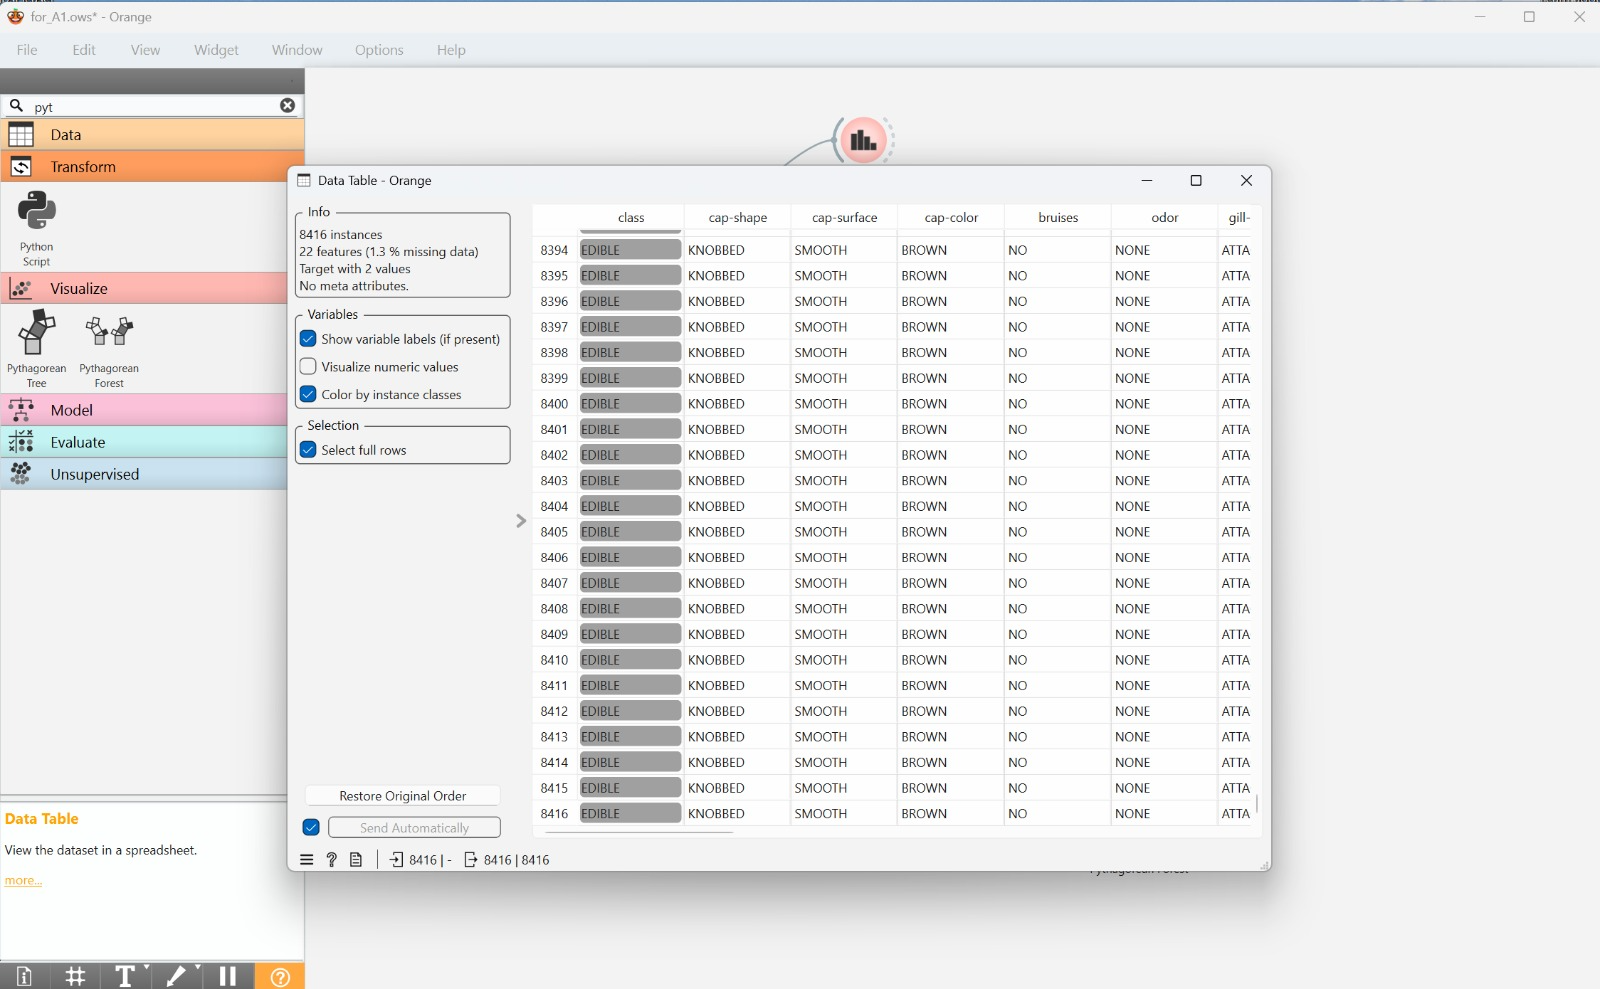
\includegraphics[width=0.9\textwidth]{figures/data_table.png}
    \caption{Data table of dataset.}
    \label{fig:data_table}
\end{figure}

\subsection{Número de instâncias de cada classe}

The FungiDataset has a distribution with 4488 instances classified as EDIBLE and 3928 instances classified as POISONOUS as can be seen in the figure below.

\begin{figure}[H]
    \centering
    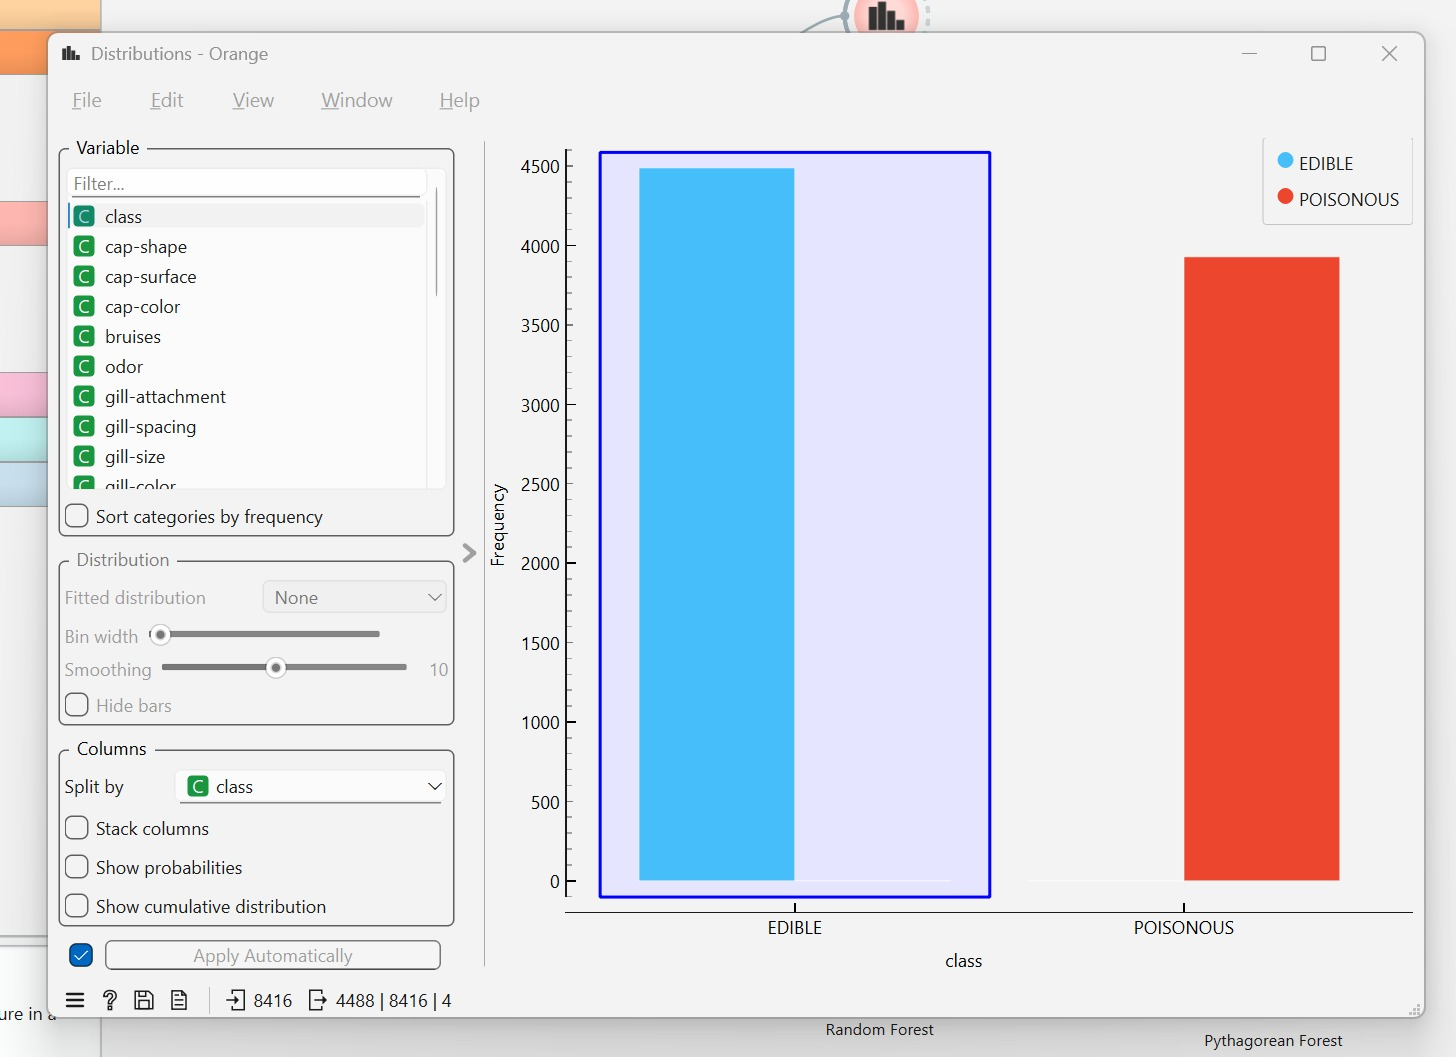
\includegraphics[width=0.7\textwidth]{figures/distribution_classes.png}
    \caption{Distribution of classes.}
    \label{fig:distribution_classes}
\end{figure}

\subsection{Classificador Tree}

Figure~\ref{fig:tree_classification} shows the result of the TREE classification using Orange. It can be observed that it chose the same parameter as 1R, correctly identifying all poisonous mushrooms and only missing 2.5\% of the edible ones (false negatives). The decision tree easily separates mushrooms because the odor attribute is a strong predictor. Subsequent splits only refine borderline cases.

\begin{figure}[H]
    \centering
    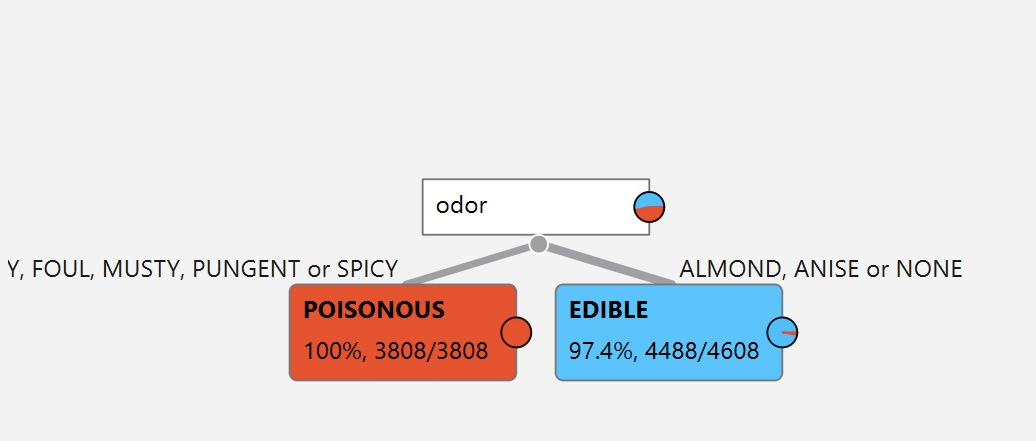
\includegraphics[width=0.8\textwidth]{figures/tree_classification.png}
    \caption{Result of Tree classification.}
    \label{fig:tree_classification}
\end{figure}

\subsection{Classificador Random Forest}

The Random Forest classifier demonstrates absolute effectiveness in correctly classifying all occurrences into their respective classes. Figure~\ref{fig:rf_confusion_matrix} perfectly illustrates the confusion matrix on the diagonal. Random Forest aggregates multiple decision trees for more stable predictions.

\begin{figure}[H]
    \centering
    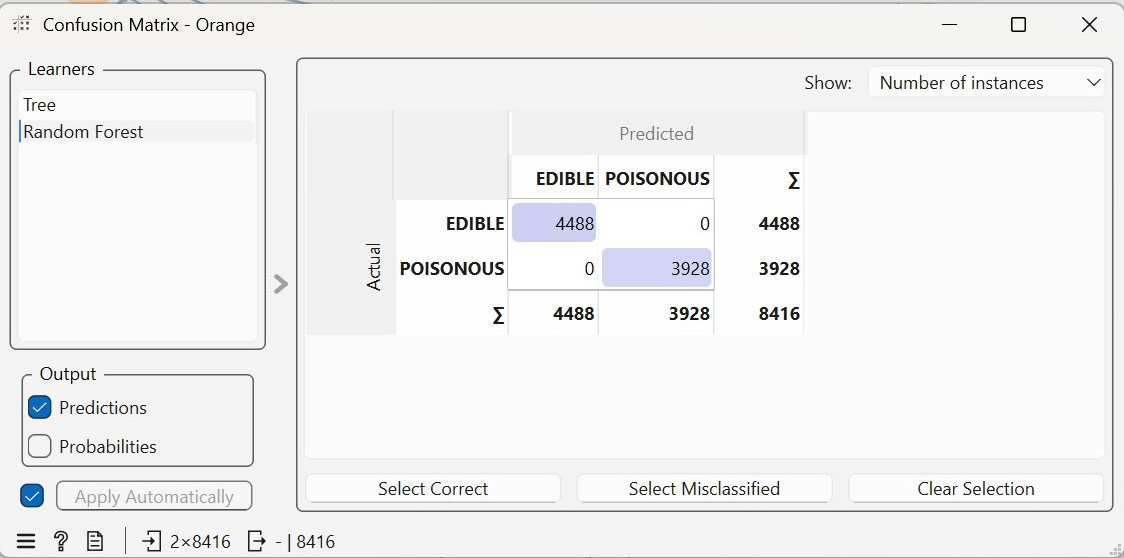
\includegraphics[width=0.7\textwidth]{figures/confusion_matrix_random_forest.png}
    \caption{Confusion Matrix of Random Forest.}
    \label{fig:rf_confusion_matrix}
\end{figure}

The fact that this classifier performed better than the previous one is due to its better distribution of training and test data, as well as its reliance on multiple decision trees. The figure below shows the trees it generated.

\begin{figure}[H]
    \centering
    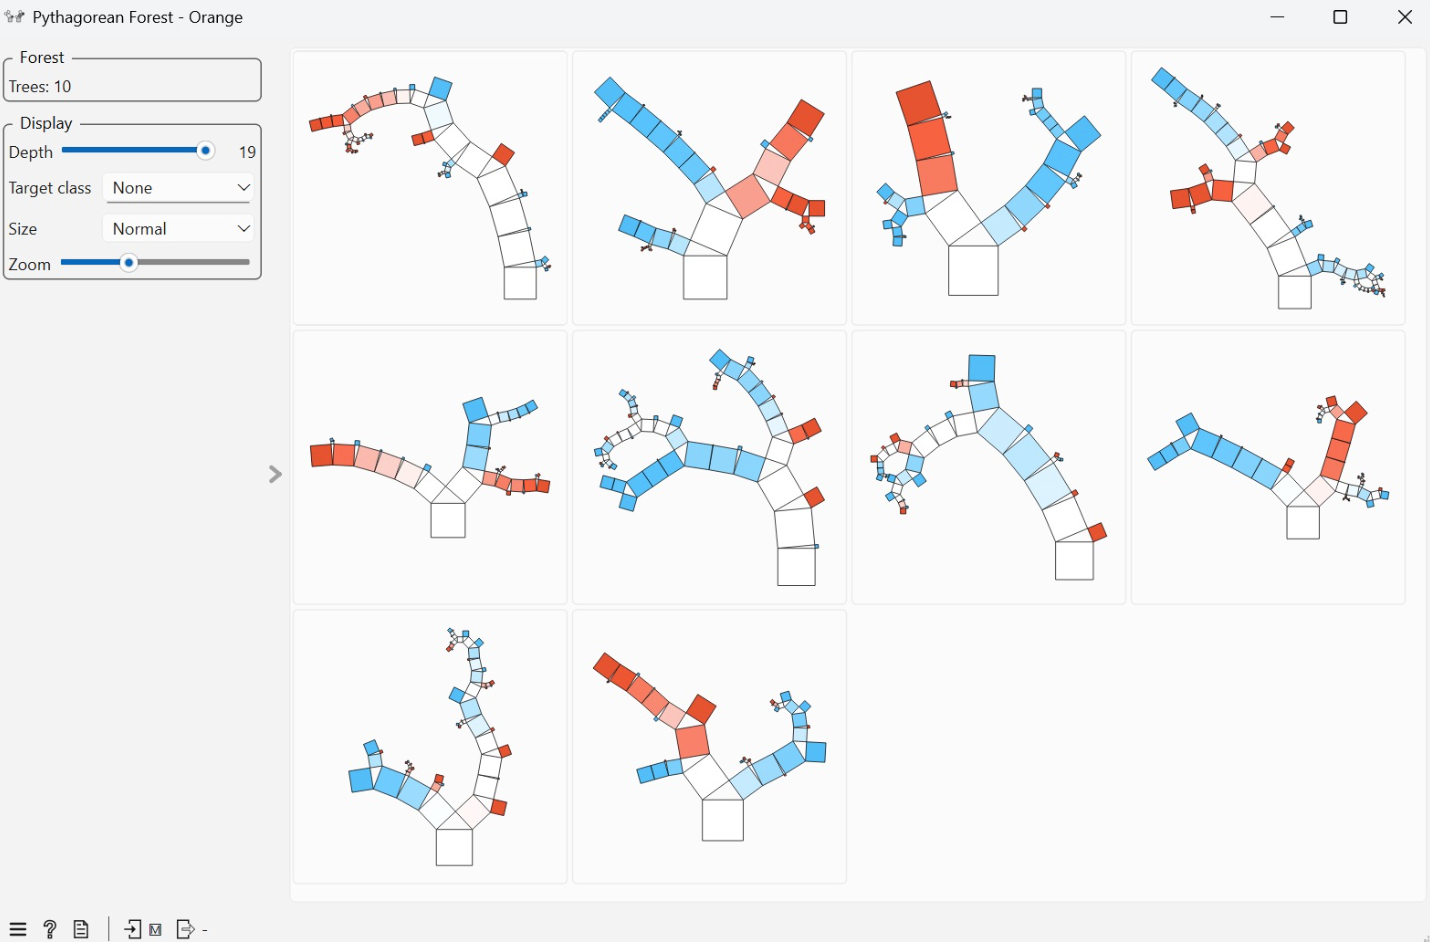
\includegraphics[width=0.9\textwidth]{figures/pythagorean_forest_map.png}
    \caption{Pythagorean Forest map.}
    \label{fig:pythagorean_forest}
\end{figure}

\subsection{Previsões}

The comparisons made are between the Tree classifier (Figure~\ref{fig:tree_confusion_matrix}) and the Random Forest (Figure~\ref{fig:rf_confusion_matrix}). As mentioned in the previous paragraph, RF has a perfect score, correctly identifying all classes; however, tree has a small deviation.

\begin{figure}[H]
    \centering
    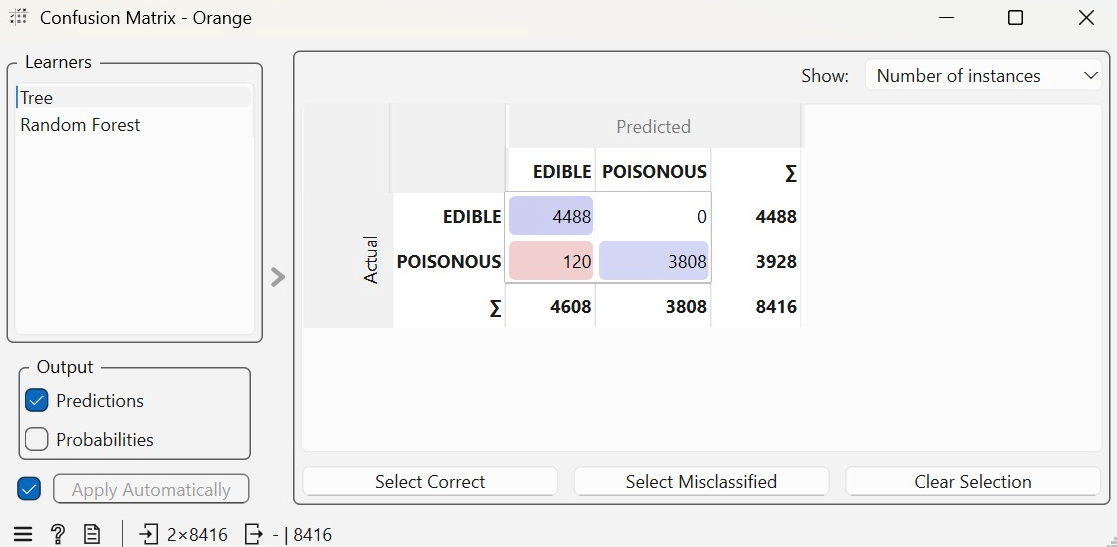
\includegraphics[width=0.7\textwidth]{figures/confusion_matrix_tree.png}
    \caption{Confusion Matrix of Tree.}
    \label{fig:tree_confusion_matrix}
\end{figure}

\section{Conclusão}

A realização deste laboratório permitiu aplicar de forma integrada várias competências desenvolvidas ao longo da unidade curricular: análise de datasets reais, preparação e transformação de dados, implementação e utilização de classificadores simples como o 1R, e exploração de modelos mais avançados em Orange Data Mining.

A utilização combinada de código e ferramentas visuais evidencia a complementaridade entre abordagens programáticas e ambientes de data mining interativos.

The mushroom dataset contains 8416 instances. The attribute odor dominates the classification. Random forest confirms robustness of predictions. Both were near perfect score with Random Forest having a slight more accurate prediction.

\end{document}
